% Chapter 3 - Methodology

% \glsresetall % reset the glossary to expand acronyms again
\chapter[Distributed Deep Learning]{Distributed Deep Learning}\label{ch:DistributedDL}
\index{Distributed Deep Learning}
Over the past decade, machine learning, and specifically deep learning (DL), has exploded in popularity.
Several incredibly challenging problems have recently been solved using emerging techniques, traditional examples include computer vision \cite{Krizhevsky2012AlexNet} and natural language processing \cite{Vaswani2017AttentionTransformer}, but more traditional scientific HPC fields like climate modelling \cite{Ham2019DLENSOForcasts} and cosmology \cite{Mathuriya2019Cosmoflow} are starting to adopt DL methods.
There is an incredible demand for DL as both academia and industry rush to develop new models to solve more problems; however, DL is an incredibly computationally intensive task, and depending on the number of model parameters and the dataset size, training time can span from hours to weeks.
To address these issues, DL practitioners are adopting HPC techniques to parallelize the training process at a massive scale and build larger models faster.
Parallelization strategies are diverse, but the three methods used at scale are hyperparameter search for evaluating different architectures, model parallelism to stretch a model across multiple nodes, and data parallelism to process multiple samples concurrently and lower time to convergence.
Data parallelism is by far the most well-understood parallelization strategy, having existed long before the recent AI revolution \cite{Zhang1990BPonCM2}, it is relatively easy to deploy, has a well-understood communication pattern, and is highly scalable.

The rest of this chapter contains a high-level overview of current distributed DL practices with a focus on data-parallel strategies, we then outline the state-of-the-art tools used at scale and investigate HPC methods that have been able to accelerate data-parallel training in literature.

\section{Deep Learning}
Deep learning is a supervised learning technique where a model is trained to approximate some ground truth source, typically a dataset.
Formally, deep learning training tries to find a function $f: X\longrightarrow Y$ which maps data from sample space $X$ to label space $Y$.
To predict how accurate $f$ is for a sample $x$, we define a loss function $L_D(f)=\mathbb{P}[f(x)\neq h(x)]$, where $x$ is a sample in dataset $D$ with label $h(x)$.
In practice, $f$ will belong to a class of function $\mathcal{H}$ containing functions $f_w$, where $w$ is a vector of parameters.
To train a model, a training algorithm will try to find some value for $w$ which minimizes the loss function of $f$ over $D$, formally:
\begin{equation}
    \argmin_{w\in\mathcal{H}} L_D(f_w) = \argmin_{w\in\mathcal{H}} \mathbb{E}_{x\in D}[\ell (w,x)]
    \label{eq:argmin-loss}
\end{equation} 
Where $\ell:\mathcal{H}\times X\longrightarrow \mathbb{R}^+$ is the loss function for an individual sample. 

Many optimization algorithms can solve equation \ref{eq:argmin-loss}, but the most widely adopted algorithm is minibatch stochastic gradient descent.
Standard gradient descent relies on a continuous optimization space, but the dataset is not a continuous space, therefore, a stochastic method is used \cite{Robbins1951StochasticAproxmethod}.
Basic stochastic gradient decent samples one data point at a time, but on modern hardware, we can increase device utilization and throughput by sampling multiple data points using a batch method \cite{Le2011OnOptMethodsforDL}.

\begin{algorithm}
    \caption{Minibatch SGD}
    \label{alg:MinibatchSGD}
    \begin{algorithmic}[1]
        \For {t = 0 \textbf{to} $\frac{|D|}{B}*epochs$} \Comment{for a specified number of iterations over the dataset}
        \State $\Bar{x}\leftarrow$ Vector of $B$ Random elements from $D$ \Comment{Take minibatch from dataset}
        \State $w_{mb}\leftarrow w^{(t)}$ \Comment{Load weights}
        \State $f\leftarrow \ell(w_{mb},\Bar{x},h(\Bar{x}))$ \Comment{Forward evaluation with minibatch}
        \State $g_{mb}\leftarrow \nabla \ell(w_{mb}, f)$ \Comment{Backpropogate to calculate gradient}
        \State $\Delta w \leftarrow u(g_{mb}, w^{(0,...,t)}, t)$ \Comment{Calculate weight update, performs allreduce}
        \State $w^{(t+1)}\leftarrow w_{mb} + \Delta w$ \Comment{Apply weight updates to next itteration}
        \EndFor
    \end{algorithmic}
\end{algorithm}

Minibatch SGD (algorithm \ref{alg:MinibatchSGD}) iterates over the dataset a predefined number of times, but other stopping criteria can include an evaluation threshold on an external validation dataset or a collapse in the loss function.
A batch of data is sampled from the training dataset in line 2, the dataset is shuffled between epochs to generate different minibatches for each epoch.
The minibatch samples are propagated through the model in the forward pass on line 4, and the set of forward pass results is used to calculate a set of gradients in line 5. 
Line 6 uses an update function to calculate the weight updates, this function is responsible for combining the gradients of all the samples into weight updates to be applied to the next iteration of the model (line 7).

While this algorithm seems simple, the research space is massive, spanning from the model's architecture to tweaking parts of the training algorithm, and there are several gotchas to watch out for.
It is possible for the optimization space to have multiple minimums, so researchers have proposed techniques to help find global minimums. 
The update calculation is essential, and the model will not converge if not properly managed, if update steps are too large, the model will not generalize and will be unstable, but if updates are too small, then training can take an exceedingly long time.
Weight initialization is one angle to tackle these issues since the final accuracy can be heavily influenced by $w^{(0)}$, initialization methods include random values, informed decisions, or transfer learning from other pre-trained models \cite{Glorot2010XavierInitalization}.
The weight update rule $u$ has also undergone a lot of research.
The most straightforward rule, $u_{sgd}(g)=-\eta \cdot g$, simply multiplies the gradient by a learning rate $\eta$, but the learning rate can be changed over time, with a common practice of exponentially shrinking the gradient with larger values of $t$.
The update rule can also include momentum, which uses the difference between current and past weights to influence update magnitude, and modern methods, like Adam \cite{Kingma2015Adam}, leverage the first and second moments of the gradient to update learning rates individually for each weight in the model.

The model's architecture also plays an important role.
The founding idea for neural networks was to approximate the structure of neurons in the brain mathematically.
Individual neurons take a set of inputs, calculate a weighted sum across a set of weights, apply an activation function to introduce nonlinearity, and pass the output on to other neurons. 
Neurons are organized into layers, often structured in a fully connected manner where the output of one neuron is connected to every neuron in the next layer.
The number of neurons in a layer defines the model's width, and the number of layers in the model defines the depth.
These early feed-forward networks have a powerful ability to learn non-linear relationships while being efficient to implement using general matrix matrix multiplications (GEMM).
However, different layer types have been proposed which can extract different features from different types of data, popular examples include convolutional layers for images \cite{Krizhevsky2012AlexNet}, recurrent layers for sequence data \cite{cho2014PhraseRepresentationRNN}, and transformer layers for text \cite{Vaswani2017AttentionTransformer}.
Further, many different activation functions can be used, with popular choices including sigmoid and rectified linear units \cite{Nair2010ReLU}.

However, one prevalent trend of DL (in fact, this is where the 'deep' in \textit{deep learning} comes from) is that larger models and larger datasets give better performance \cite{Kaplan2020ScalingLawsForNLModels, Ben-Nun2019DemystifyDL}.
There is a consistent trend of larger models training on larger datasets, however, the more these factors scale so does the required training time.
To address these issues, several parallelization strategies have been applied.
Individual layer operations were the initial target for optimization, and many hardware providers have released software libraries designed to run layer-specific operations like convolutions and GEMM as fast as possible, examples include Intel's MKL and Nvidia's CUDNN \cite{MKL, cuDNN}. 
The compute-intensive nature of DL models has led to the wide adoption of GPUs as the massively parallel capabilities of these accelerators can blast through training and inference orders of magnitude faster than CPUs.

GPUs still have a limit to how many TFLOPs they can drive, and there are limits to the amount of accelerator memory, but both of these limits can be broken by scaling across a cluster.
So this thesis focuses on DL parallelization across GPU clusters.
Some problems can't fit into a single GPU or even a single node with multiple GPUs, and a multi-node distributed training strategy needs to be adopted.
There are common strategies for parallelizing deep learning, each has its own benefit, and often, multiple of these strategies can be combined.

\section{Parallel Deep Learning}

\subsection{Hyperparameter search}
The features specifying a DL model can be lumped into two categories, parameters and hyperparameters.
Parameters are values that are filled by the optimization algorithm and are essentially a synonym for the model's weights, while hyperparameters focus on specifying the structure of the model and remain unchanged during training.
Hyperparameters include structural features of the model like the number and types of layers, activation functions, and the loss function, and they can also extend to the training algorithm with tunables like learning rate, learning rate decay, and batch size.
The setup has an outsized impact on model performance, so often, a lot of model development time goes into hyperparameter selection, however, each new hyperparameter add another search dimension and exponentially increases the search space.
Therefore, automated hyperparameter search strategies are a popular target for parallelization at scale.

Hyperparameter search is incredibly compute-intensive and does not generate that much communication, which makes it a great candidate for parallelization.
Initially proposed search algorithms include sequential search heuristics, like grid search \cite{Hadjis2016Omnivore}, where a series of candidates are identified, models are trained for each, and the search space is iteratively refined based on the training results.
More clever techniques could use evolutionary algorithms \cite{Young2017EvolveNLWithHPC, Real2017LargeScaleEvolutionOfCV}, which generates a population of candidate models and iteratively removes underperforming models and replaces them with higher-performing models with random perturbations, or reinforcement learning \cite{Zoph2017NeuralArchSearchReinformceLearn} which uses gradient-based optimization to discover more optimal model architectures.
Large-scale hyperparameter search systems are often based on a parameter server/worker design, where the parameter server manages the search algorithm and issues models for worker nodes to train and evaluate.
These systems generate relatively little communication as model architectures can be specified in a few bytes, workers can take hours to train a model, and they have been relatively easy to scale to exceedingly large systems \cite{Young2017EvolveNLWithHPC}.

\subsection{Model Parallelism}
\begin{figure}
    \centering
    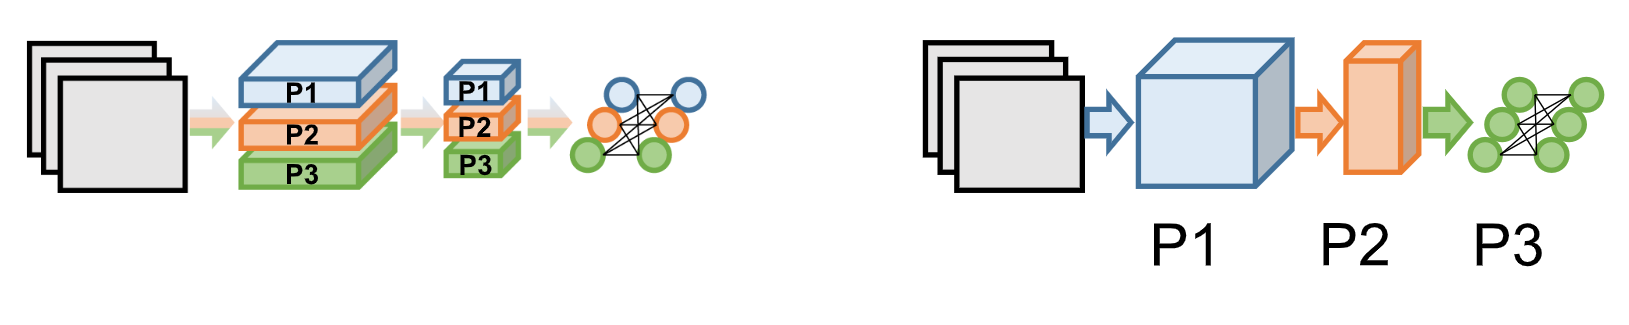
\includegraphics[width=15cm]{3_Chapters/3_Chapter_DistributedDL/Figs/model_parallel_decomposition.png}
    \caption{Tow methods for partitioning a neural network,  left is spacial decomposition right is layer-wise.}
    \label{fig:model-parallel-decomposition}
\end{figure}
Model parallelism splits the model's architecture into chunks and distributes partitions across processing resources.
There are multiple decomposition strategies, but the two most general ones are decomposition by layer and spatial decomposition, both outlined in figure \ref{fig:model-parallel-decomposition}.
Layer-wise model parallelism uses individual layers as units for work and issues one or more layers on each processing resource \cite{Abadi2015TensorflowWhitepaper}. 
Spatial decomposition takes a finer-grained approach, it breaks individual layers into sections and can map a single layer across multiple ranks \cite{VanEssen2015LBANN}.
It is also possible for both strategies can be used in parallel, which provides flexibility to map network elements to compute to maximize machine utilization \cite{Dean2012DistBelif}.

The critical benefit of model parallelism is how it removes model size scaling limits.
The amount of available memory often limits the number of model parameters, but these techniques allow networks to access a larger memory pool.
However, the added complexity of a distributed memory environment can add several complications to model design. 
Layer-wise decomposition can introduce 'bubbles' of idle time, the forward pass must be complete before weight updates can be calculated, forcing ranks earlier in the network to stall as deeper ranks complete their work \cite{Huang2019Gpipe}.
Connections between layers can generate all kinds of complicated data exchange patterns, spatially decomposed networks can introduce halo-exchanges for layer inputs, and layer-decomposition can introduce all-to-all collectives across fully-connected layers \cite{Coates2013DLwithCOTSHPC, Dryden2019ImprvScaleofCNN}.
These drawbacks add a lot of complexity to the design of model-parallel networks, and the added communication can potentially ruin scalability if not adequately accounted for.

\subsection{Data paralleism}
\begin{figure}
    \centering
    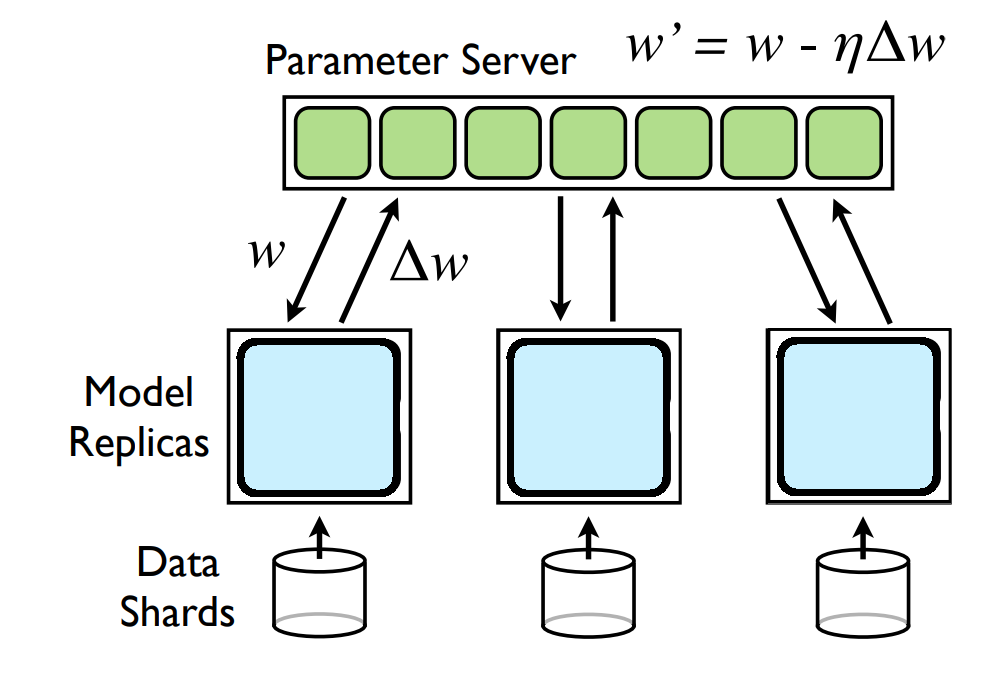
\includegraphics[width=10cm]{3_Chapters/3_Chapter_DistributedDL/Figs/parameter_server.png}
    \caption{Parameter server, taken from \cite{Dean2012DistBelif}}
    \label{fig:parameter-server}
\end{figure}

\begin{figure}
    \centering
    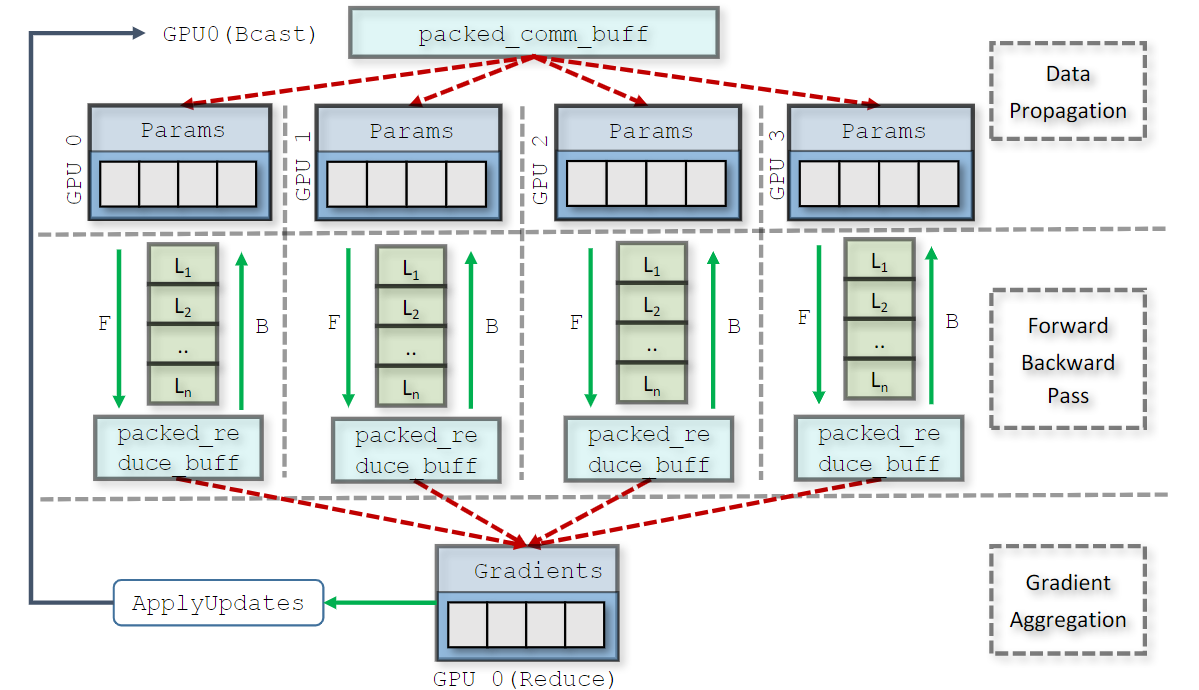
\includegraphics[width=15cm]{3_Chapters/3_Chapter_DistributedDL/Figs/Caffee_DP_arch.png}
    \caption{Data parallel architecture of Caffe, taken from \cite{Awan2017InDepthPerfCharOfDNN}}
    \label{fig:caffe-dp-arch}
\end{figure}
Recall that in minibatch SGD, samples within a batch are not computationally dependent on each other, data parallelism leverages this fact to evaluate multiple samples within a minibatch concurrently and speed up the time to evaluate an epoch. 
Each process performs a forward and backward pass on a subset of the minibatch and calculates a local weight update, and the global average of all weight updates is applied to the model for the next epoch.
However, there are mathematical challenges to scaling, adding more processes implicitly increases the batch size, which impacts the model's final convergence, and larger batch sizes tend to perform poorly \cite{Keskar2016LargeBatchTraining}.
To combat this, researchers have found that appropriately tuned update rules and regularization layers, like batch normalization, improve large batch training \cite{You2018ImgNetInMin, Goyal2017FacebookImgNet1Hour}. 

The other challenge is the added communication.
$\delta w$ needs to be identical across all ranks, this adds some form of synchronization to every epoch and can become the scaling bottleneck if not accounted for.
The first forays into large-scale data-parallel deep learning were built around centralized parameter server \cite{Dean2012DistBelif, Chilimbi2014ProjectAdam}.
This architecture, outlined in figure \ref{fig:parameter-server}, designates a coordinator process to manage the global state of the model, and issue weights and minibatches to workers which calculate weight updates in parallel, then return their $\delta w$ to the server who updates the model for the next round.
This design is fault-tolerant, workers can drop out, and training can continue without hiccups. 
The parameter server can also be extended to a hierarchical server pool, providing more resiliency and bandwidth. 
However, the fatal flaw of this design is how the server can become a performance choke point.
Using communication modelling established in Section \ref{sec:CH2-MPI-AlgStructure}, a singular server would need to receive $p$ messages and perform $p$ reductions, introducing a whopping communication cost of $p(\alpha+n(\beta+\gamma))$.
Synchronization can be relaxed at an algorithmic level by lowering the required model consistency, some methods only send $\delta w$ and periodically refresh their local copy of the model to not deviate too far \cite{Dean2012DistBelif}, while others altogether remove any synchronization and rely on the sparse nature of $w$ to mitigate race conditions \cite{Noel2014Dogwild}.
SGD is resilient to model disruptions and can still converge even if work is lost due to synchronization errors. 
However, parameter servers training is still not scalable enough to reach exascale.

To elimitate the parameter server a decentralized approach must be taken.
To acomplish this, the parameter server's jobs of aggregating, averaging, and distributing the model update  can be replaced by an allreduce operation.


\cite{Sergeev2018Horovod}.
\cite{Kurth2019TFatScaleAnalysisOfHvdAndCPEML}
\cite{Mathuriya2019Cosmoflow}
\cite{Ham2019DLENSOForcasts}

\cite{Awan2017SCaffe}

\begin{itemize}
    \item Math foundation of Distributed DL, \cite{Ben-Nun2019DemystifyDL}
    \item Lit review of DL (Awan's work + more), establish that Allreduce is Key
    \item Existing Deep learning libraries (Tensorflow, Pytorch, Horovod, DeepSpeed)
    \item Potentially some DL profiling (Python based)
\end{itemize}



\clearpage